\section{DDC Traffic Characterization}
\label{sec:workloads}
In this section, we explore the first question: characterizing the network traffic in disaggregated datacenters. We start by outlining the methodology used in our study (\S\ref{ssec:method1}). In \S\ref{ssec:flc}, we discuss the flow-level characteristics (flow size distribution, inter-arrival times, etc.). We then discuss network-level traffic characteristics in \S\ref{ssec:nlc}, including traffic volume, spatial and temporal distribution. We close the section with a discussion on how various design knobs from \S\ref{sec:summary} impact our observations regarding the flow-level and network-level characteristics of traffic in disaggregated datacenters (\S\ref{ssec:knobs}).

Broadly, our results show that
\begin{itemize}
\item The flow size distribution in \dis is more homogeneous --- that is, compared to \pdis, flows are distributed over a smaller range.
\item For most applications, both the number of flows and the overall traffic volume in \dis are greater than the number of flows in \pdis.
\item While in \pdis the traffic volume is spread over all source-destination pairs, in \dis a number of such pairs have no traffic between them --- that is, the traffic matrix changes from all-to-all to some-to-some.
\item \rqc{stuff from yet-to-be-written 4.4}
\end{itemize}

%
\begin{figure}
	\centering
	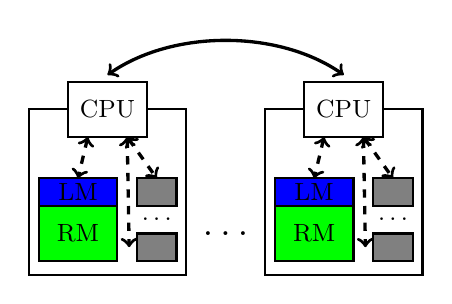
\begin{tikzpicture}[xscale=0.5, yscale=0.35]

	\draw[very thick, black, <->] (-1, 12.25) to [out=45, in=135] (5, 12.25);

	\draw[thick, fill=white] (-3, 5) rectangle (1, 11); 
	\draw[thick, fill=white] (-2, 12) rectangle (0, 10); 
	\draw (-1, 11) node {\small{CPU}};
	% \draw (-1, 10.5) node {\small{Handler}};
	
	\draw[thick, fill=blue] (-2.75, 7.5) rectangle (-0.75, 8.5);
	\draw[thick, fill=green] (-2.75, 5.5) rectangle (-0.75, 7.5);
	\draw (-1.75, 8) node {\small{LM}};
%	\draw (-2.75, 7.5) -- (-0.75, 7.5);
	\draw (-1.75, 6.5) node {\small{RM}};
%	\draw (-2.75, 6.5) -- (-0.75, 6.5);
%	\draw (-1.75, 6) node {\small{K$\to$O}};

%	\draw[thick] (-0.25, 5.5) rectangle (0.75, 8.5);
	\draw[thick, fill=gray] (-0.25, 8.5) rectangle (0.75, 7.5);
	\draw[thick, fill=gray] (-0.25, 5.5) rectangle (0.75, 6.5);
	\draw (0.25, 7) node {\small{$\dots$}};

	\draw[very thick, black, dashed, <->] (-1.5, 10) -- (-1.75, 8.5);
	\draw[very thick, black, dashed, <->] (-0.5, 10) -- (0.25, 8.5);
	\draw[very thick, black, dashed, <->] (-0.5, 10) -- (-0.45, 6);

	\draw (2, 6.5) node {\Large{$\dots$}};

		\draw[thick, fill=white] (3, 5) rectangle (7, 11); 
		\draw[thick, fill=white] (4, 12) rectangle (6, 10); 
		\draw (5, 11) node {\small{CPU}};
		% \draw (5, 10.5) node {\small{Handler}};

		\draw[thick, fill=green] (3.25, 5.5) rectangle (5.25, 7.5);
		\draw[thick, fill=blue] (3.25, 7.5) rectangle (5.25, 8.5);
		\draw (4.25, 8) node {\small{LM}};
		\draw (4.25, 6.5) node {\small{RM}};

	%	\draw[thick] (-0.25, 5.5) rectangle (0.75, 8.5);
		\draw[thick, fill=gray] (5.75, 8.5) rectangle (6.75, 7.5);
		\draw[thick, fill=gray] (5.75, 5.5) rectangle (6.75, 6.5);
		\draw (6.25, 7) node {\small{$\dots$}};

		\draw[very thick, black, dashed, <->] (4.5, 10) -- (4.25, 8.5);
		\draw[very thick, black, dashed, <->] (5.5, 10) -- (6.25, 8.5);
		\draw[very thick, black, dashed, <->] (5.5, 10) -- (5.55, 6);

	\end{tikzpicture}
	    \caption{\small{We run real-world applications on a $5$-node Amazon EC2 cluster and emulate disaggregated architecture as follows. The memory accesses are captured into ``local cache'' accesses and ``remote memory'' accesses using an in-house implementation of a special instrumentation tool (SIT) described in \S\ref{sec:workloads}. The local disk accesses are captured using the {\tt blktrace} utility. Finally, all remote memory and disk accesses are captured using {\tt TCPdump}.}}
	\label{fig:system2}
\end{figure}
%
\subsection{Methodology}
\label{ssec:method1} 
To characterize the traffic in disaggregated datacenters, we set up a testbed comprising of $5$ Amazon EC2 \texttt{m3.2xlarge} machines running Amazon Linux, each with $16$ vCPU, $32$GB of main memory, $1$TB of magnetic disk drives and $1$Gbps links. The Amazon EC2 machines we used were Private network enabled, ensuring no interference with other machines in the cluster. For each of the applications in Table~\ref{tab:workloads}, we capture local and remote data access flows, both for memory and disk.

\paragraphb{Inter-machine communication in \pdis}
To compare the traffic in \dis against the traditional server-centric architecture, we first characterize the flows in existing datacenters. To achieve this, we run the applications atop the above cluster. We then use {\tt TCPdump}~\cite{tcpdump}, which gives us a packet-level log of inter-machine communication. The packet-level log is combined into a flow level log by combining on the five-tuple; this approach has the limitation that the source port id a given application uses for various connections will be distinct. This is largely true except in the case of memcached, which maintains a unique port number for each client-server pair --- in this special case we limit flow sizes to the known request size of 10KB.

\paragraphb{Local and remote memory accesses in \dis}
To capture remote memory accesses, we first logically partition the main memory into ``local cache'' and ``remote memory''; for reasons described later, we use $30\%$ of the main memory as local cache. We then use an in-house implementation of a light-weight special instrumentation tool (SIT), implemented as a shim layer between the CPU and the swap device. The SIT intercepts all page faults, or memory access requests into the part of main memory identified as remote, and records the time and address accessed. Consequently, all captured requests are at page granularity and ergo have the same size (4KB). Memory requests arrive at SIT in batches; these batches are grouped into flows for \dis.

\paragraphb{Disk accesses in \dis}
We capture disk accesses during application runtime using the {\tt blktrace} utility, which provides disk access traces at the granularity of disk block sizes. Note that the data residing on a single disk is not necessarily on consecutive disk blocks (due to disk fragmentation); thus, a single file access from the disk may result in accessing non-consecutive disk blocks. Since {\tt blktrace} provides disk access patterns at the disk block granularity, it is impossible to infer which disk block accesses correspond to a single disk access request at the application layer. We, thus, use a simple heuristic to combine multiple disk block access into a single application layer request --- all those disk block accesses that occur within a small $\delta$ time range are combined into a single disk access. We study the sensitivity of our results against $\delta$ during traffic characterization. 

It is important to note the mapping of \pdis flows to \dis flows. \pdis flows represent remote reads (\ie shuffle traffic); these reads are captured as \emph{local} reads in \dis on the machine where the data was located. Therefore, to accurately represent traffic in \dis we must attribute some fraction of reads to a given disk to a CPU blade other than the one the disk read was recorded on. To do so we match disk flows with NIC traffic by time. If a disk flow is matched to a NIC flow, it is assumed to be part of a remote read and it is attributed to the source of the NIC flow. Otherwise, the disk flow is assumed to be a local disk read and its source attribution is unchanged.

\paragraphb{Data placement in \dis}
All memory and disk accesses in \dis are associated with a specific address in the respective global virtual memory space. This address space is partitioned into nodes using a simple range hashing algorithm. There are five memory nodes and three disk nodes for a 5-machine ec2 cluster --- this represents the fact that disk access is slower than memory access, and thus can support more resource per blade without becoming bandwidth constrained.

Our range hashing splits the address space for memory and disk on each ec2 machine into 5 and 3 parts, respectively, to match the number of nodes for each resource type. Each range is then mapped to a resource blade, and this is repeated for each of the five ec2 machines. This mapping allows for sequential address accesses to be pipelined for greater throughput. We leave a more thorough exploration of address mapping in \dis to future work.

%Our range hashing works as follows: 
%\begin{enumerate}
%\item the address space for each node is split evenly into (number of nodes) contiguous ranges --- memory space split into 5 and disk space split into 3
%\item each range is mapped to one disaggregated node
%\item this is done for all five ec2 machines
%\item Using a range hashing algorithm allows for sequential address accesses to be pipelined for higher throughput. 
%\item We leave a more thorough exploration of this particular design knob to future work.
%\end{enumerate}

\paragraphb{Transforming data accesses into network flows}
In a disaggregated datacenter, it is possible to combine flows representing multiple requests between the same source and destination into a single flow. We use a threshold of 50 us between requests; that is, all traffic between two hosts is combined into a single flow as long as there is no intervening 50 us quiescent period. Finally, for both memory and disk flows we represent a read as a flow with its source at a memory or disk blade and its destination at a CPU, and we represent writes as flows in the opposite direction.

%However, this would require changes in the application, and possibly in network elements at the end hosts. To avoid such complications, we simply assume that each remote memory access and disk access constitutes a flow in disaggregated datacenter.

\paragraphb{Limitations}
Our instrumentation approach has two significant limitations. First, access to memory and disk accesses is only possible at page and block granularity, respectively. While we cannot explore other points in this design space, as discussed in \S\ref{sec:summary} page and block level accesses in \dis are a reasonable granularity at which to structure remote accesses in \dis. Second, accesses caused by remote flows and accesses that originated locally are indistinguishable, and thus we use a heuristic to assign disk flows to remote CPU nodes. However, we note this limitation affects only the assignment of flows to source-destination pairs, not the amount of traffic observed.

%\begin{enumerate}
%\item Our instrumentation only allows access to memory and disk accesses at page and block granularity, respectively. While as discussed earlier page-level accesses may be desirable in \dis for locality, we were unable to explore other points in the design space.
%\item Our instrumentation cannot distinguish between accesses caused by remote flows and accesses that originated locally. We are forced to use a heuristic to assign disk flows to remote CPU nodes.
%\end{enumerate}
%
\begin{figure}
  \centering
  \subfigure{
    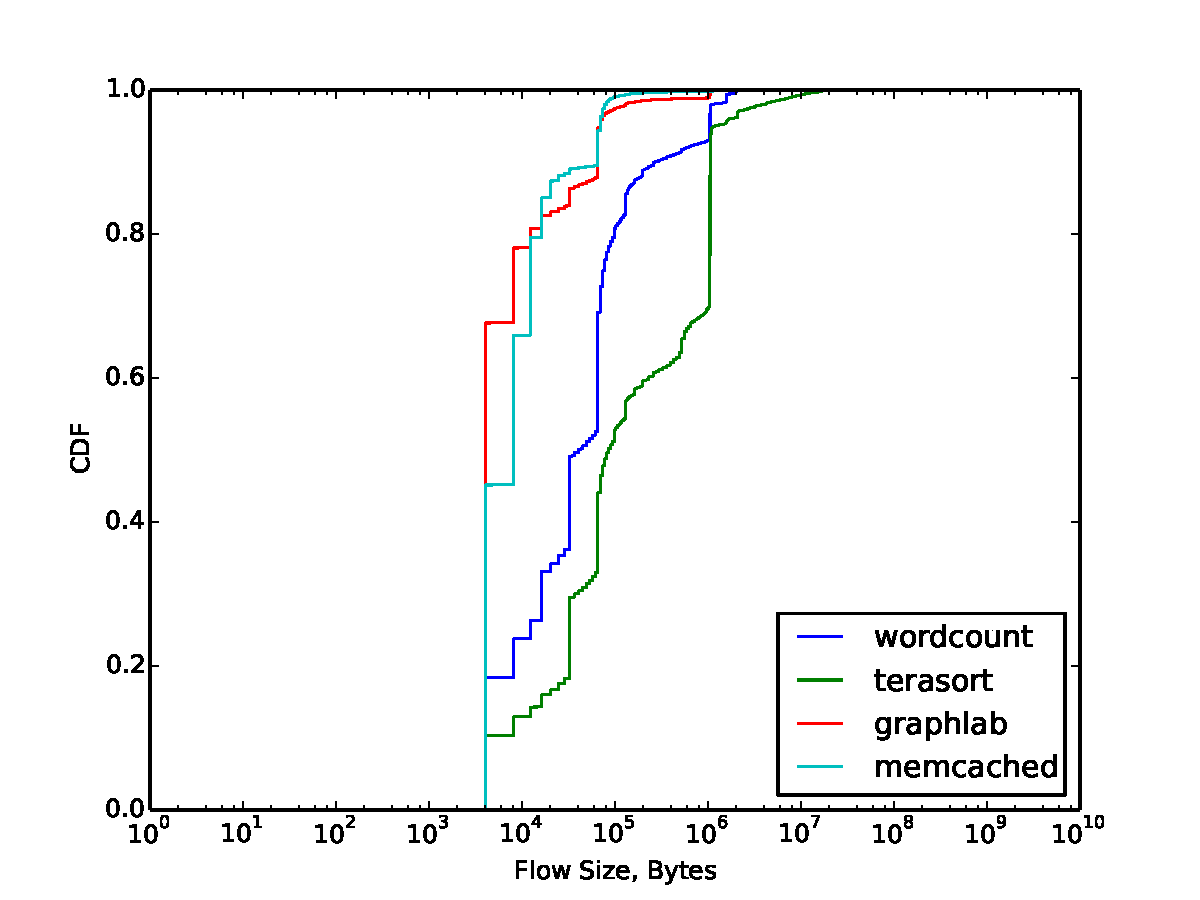
\includegraphics[width = 2.25in]{img/graph1_sizedist_dis} 
	\label{fig:asdd}
  }
%\hspace{0.05in}
  \subfigure{
    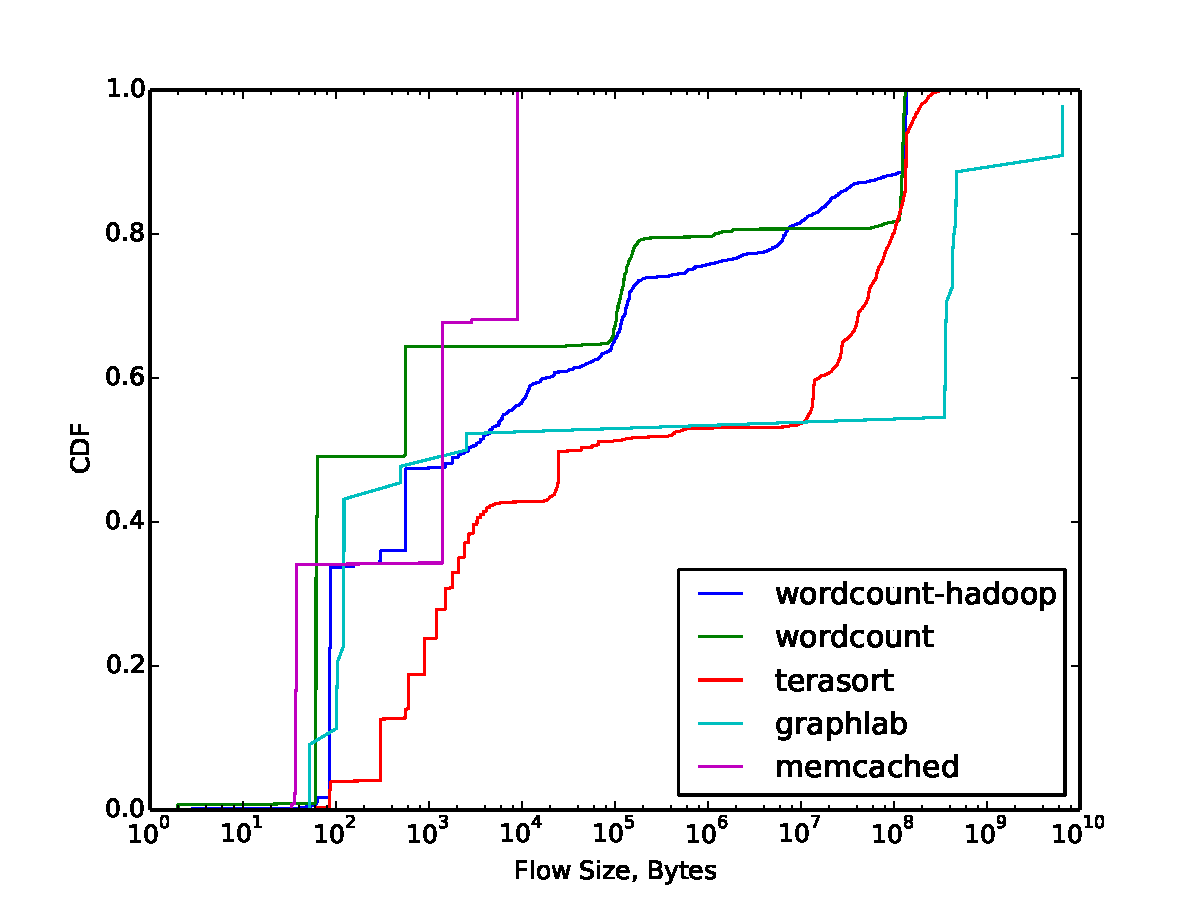
\includegraphics[width = 2.25in]{img/graph1_sizedist_pdis}
	\label{fig:sdds}
  }
  \caption{\small{Flow size distribution in \dis (above) and \pdis (below). Note that the x-axis is log-scaled.}}
  \label{fig:fsd}
\end{figure}
%

\subsection{Flow-level Characterization} 
\label{ssec:flc}
We start by discussing the flow-level characteristics in \dis, including flow size distribution, flow count and flow arrival time distribution. We then discuss some of the implications of our results regarding flow-level characterization of \dis traffic.

\subsubsection{Flow Size Distribution}
We start by discussing the flow size distribution in \dis. Figure~\ref{fig:fsd} shows the distribution of flow sizes across the six applications from Table~\ref{tab:workloads}. We make three interesting observations. First, the flow sizes are concentrated in the relatively small range [4KB, 40MB]. Second, across all the applications we evaluated, the flow size distribution is dominated by memory traffic (4KB flows) and at least $60\%$ of the flows are less than $100$KB. Finally, the tail in flow size distribution is almost non-existent, implying that irrespective of the application the elephant-mice effect typically observed in \pdis is absent.

Intuitively, the lack of short flows is because all inter-node traffic is at page granularity, and pages are 4KB long. Long flows are absent as a consequence of the data placement technique outlined in \S\ref{ssec:method1}. Overall, by enabling a more flexible placement of data, \dis will allow a more uniform distribution of flows injected into the network.

Figure~\ref{fig:fsd} also shows the flow size distribution with the same applications running atop \pdis. We note that the distributions are significantly different in \pdis --- the flow sizes span an additional two orders of magnitude both of short and on long flow sizes and the traffic is not dominated by any one particular flow size. Note that our flow size distribution in \pdis conforms with previous studies~\cite{srikanth, theo}.

%
\begin{figure}
  \centering
    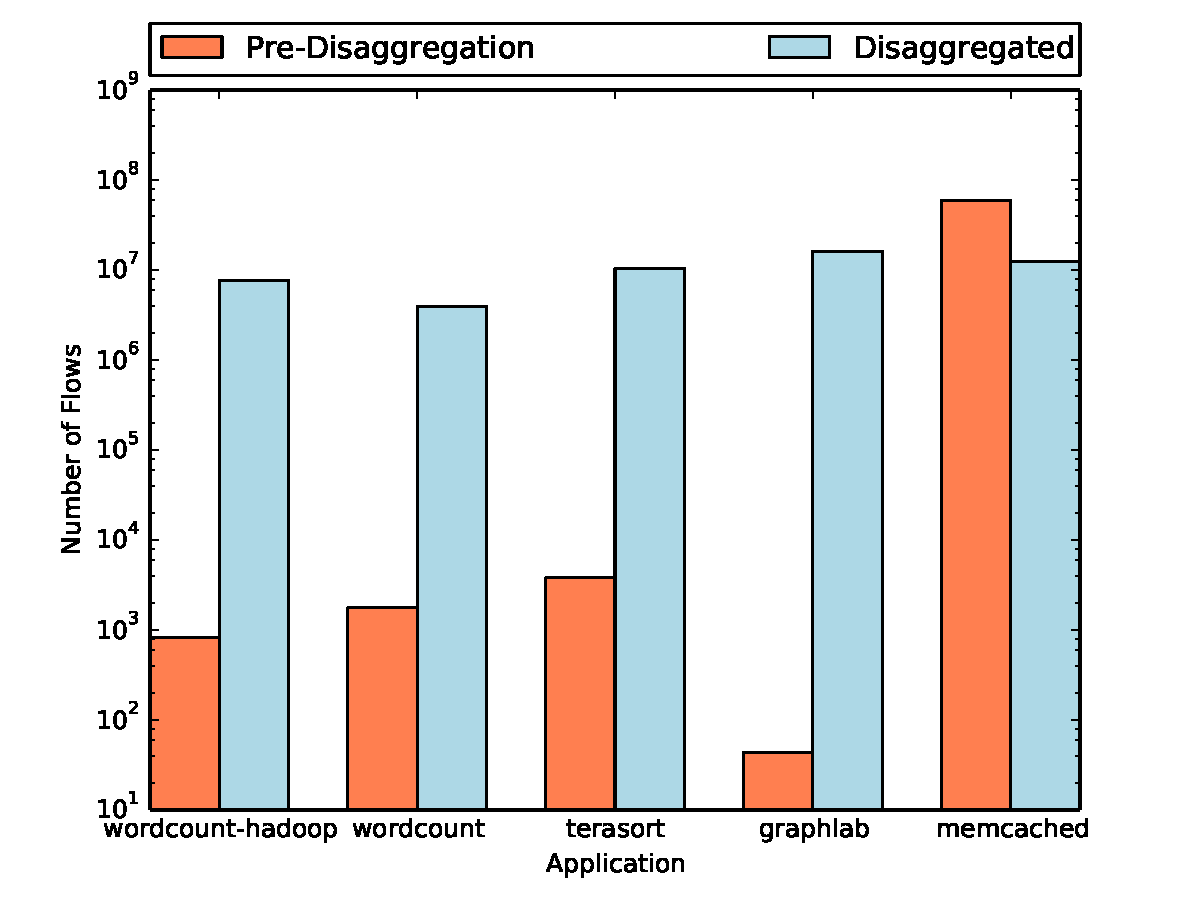
\includegraphics[width = 2.5in]{img/graph2_numflows} 
  \caption{\small{Number of flows in \dis and \pdis. Note that the y-axis is log-scaled.}}
  \label{fig:nof}
\end{figure}
%
%
\subsubsection{Flow count and volume}
\label{sssec:fctv}
Figure~\ref{fig:nof} shows that the number of flows in \dis increases by several orders of magnitude over \pdis for most applications. This is expected since a large number of disk and memory access flows that are contained within a server in \pdis (over PCIe, etc) are now injected into the network.

Interestingly, in memcached the number of flows in \dis is fewer than in \pdis. After investigation, we found that while in \pdis each request will result in a network flow, in \dis some requests are serviced by the local memory cache without crossing the network. This phenomenon is discussed further in~\S\ref{sssec:tfvol}.
%
%Figure~\ref{fig:vof} shows that the number of bytes in \dis is more uniformly distributed across short and long flows when compared to \pdis. There are two main reasons for this -- the memory flows dominating the network flows (thus having more bytes in short flows), and the long flows having been distributed across the network leading to reduction in \#bytes in long flows \rc{$\gets$ not sure about this}
%
\begin{figure}
  \centering
  \subfigure{
    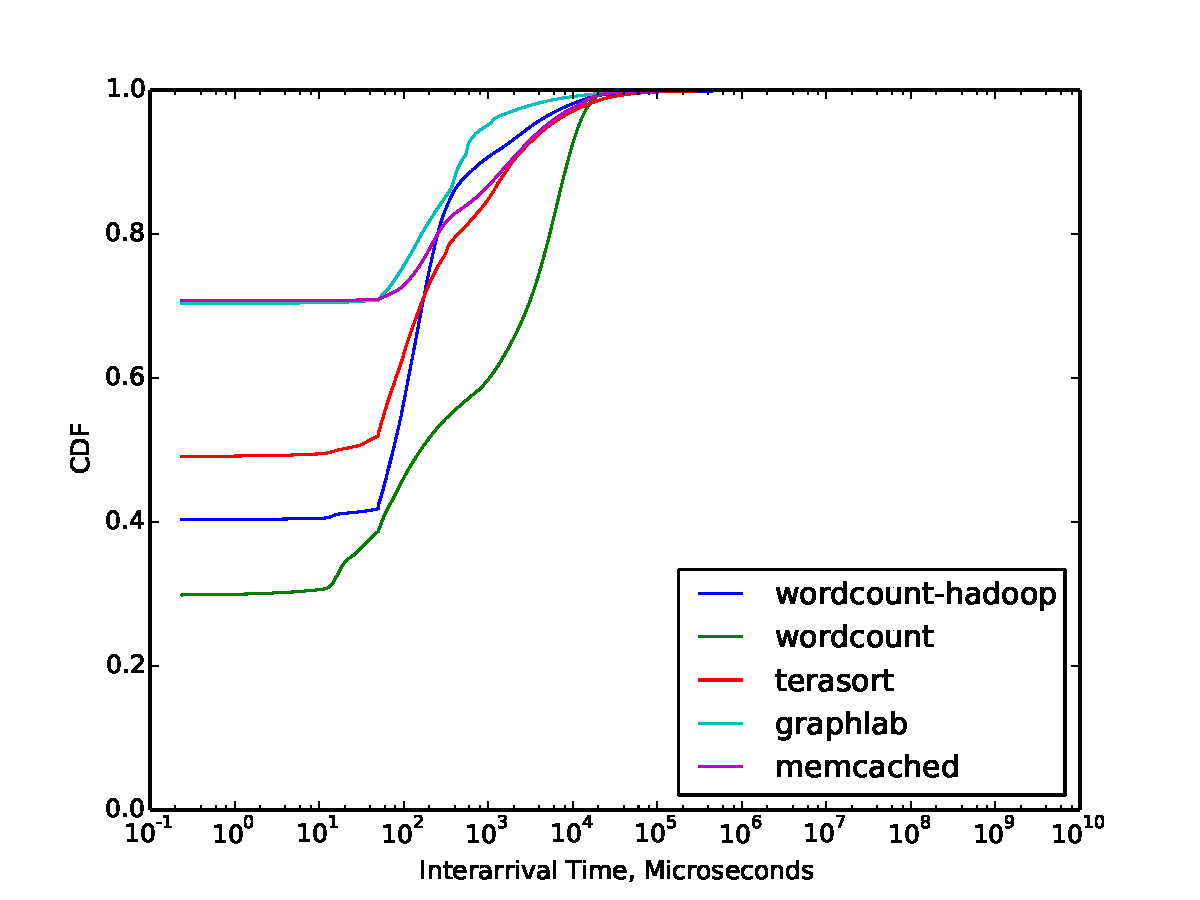
\includegraphics[width = 2.3in]{img/graph4_interdist_dis} 
	\label{fig:asdd}
  }
%\hspace{0.05in}
  \subfigure{
    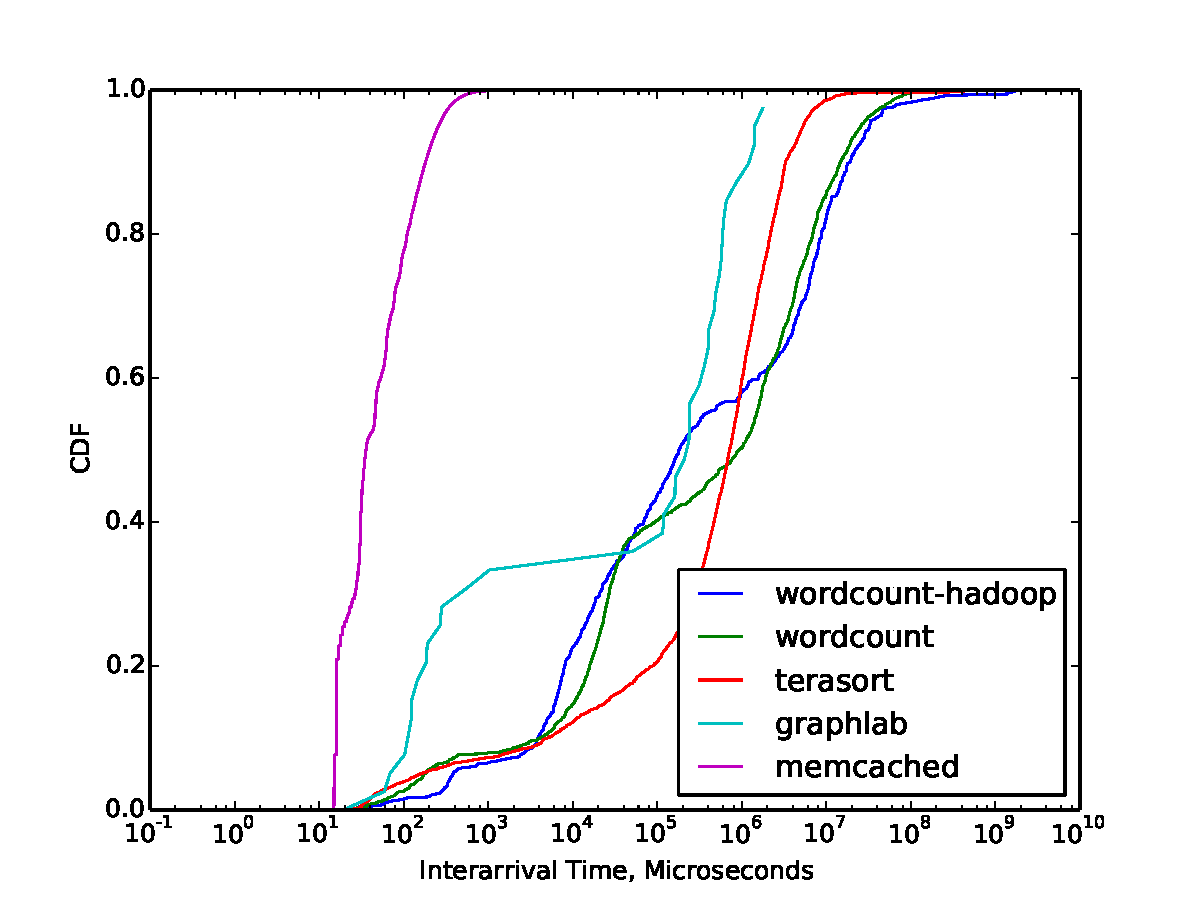
\includegraphics[width = 2.3in]{img/graph4_interdist_pdis}
	\label{fig:sdds}
  }
  \caption{\small{Flow arrival time distribution in \dis and \pdis. All the applications go into one figure: six lines in the CDF, one for each application. The same thing for \pdis.}}
  \label{fig:fat}
\end{figure}
%
\subsubsection{Flow Arrival Time Distribution}
\label{ssec:fatd}
\rc{This section along with figure 8 are slated for removal because we cannot count remote memory flows.}
Next, we study the flow arrival times in \dis. Figure~\ref{fig:fat} shows the flow arrival time distribution for the six applications from Table~\ref{tab:workloads}. We make two interesting observations. First, the flow arrival time distribution is essentially independent of the application. This is because memory access traffic dominates all the applications, leading to similar flow arrival time distribution. Second, the flow arrival time distribution is significantly different from Poisson distribution, a commonly accepted approximation to workloads in \pdis. \rc{We should say something about inter-flow arrival times --- too small? not too small? any significant different compared to \pdis?}

Figure~\ref{fig:fat} also shows the flow arrival time distribution in \pdis. As observed in several previous studies~\cite{srikanth, theo}, the distribution is very close to Poisson distribution providing a second order support to our evaluation methodology. In comparison to \pdis, the distribution is significantly different in \dis as discussed above.

\subsubsection{Implications}
Our characterization of flows in \dis allows us to draw two conclusions. First, given that \dis traffic is dominated by latency-sensitive short flows and that the number of flows increases dramatically, centralized solutions to flow scheduling may not be practical. Such solutions, if deployed in \dis, would need to dramatically lower short-flow latency as well as be able to scale up to cope with larger numbers of flows. Second, future protocols should be designed with our flow characteristics in mind --- namely, protocols should not rely on the elephant-mice conjecture for performance, and should be able to handle a more homogeneous flow size distribution. \rqc{more implications?}

%\begin{itemize}[leftmargin=*]
%	\itemsep0em
%	\item Traffic dominated by latency-sensitive short flows --- centralized flow schedulers may be inefficient
%	\item Number of flows increased --- centralized solutions may see more scalability issues
%	\item \rc{slated for removal} Flow arrival times too small --- centralized solutions inefficient
%	\item More homogeneity in flow sizes --- design of protocols
%	\item Traffic volume more uniformly distributed across short and long flows --- design of protocols
%\end{itemize}

\subsection{Network-level Characterization} 
\label{ssec:nlc}
We now study the network-level characteristics in \dis, including network traffic volume, spatial distribution and temporal distribution. We then discuss implications of our study of network-level characterization of \dis traffic.

%
\begin{figure}
  \centering
    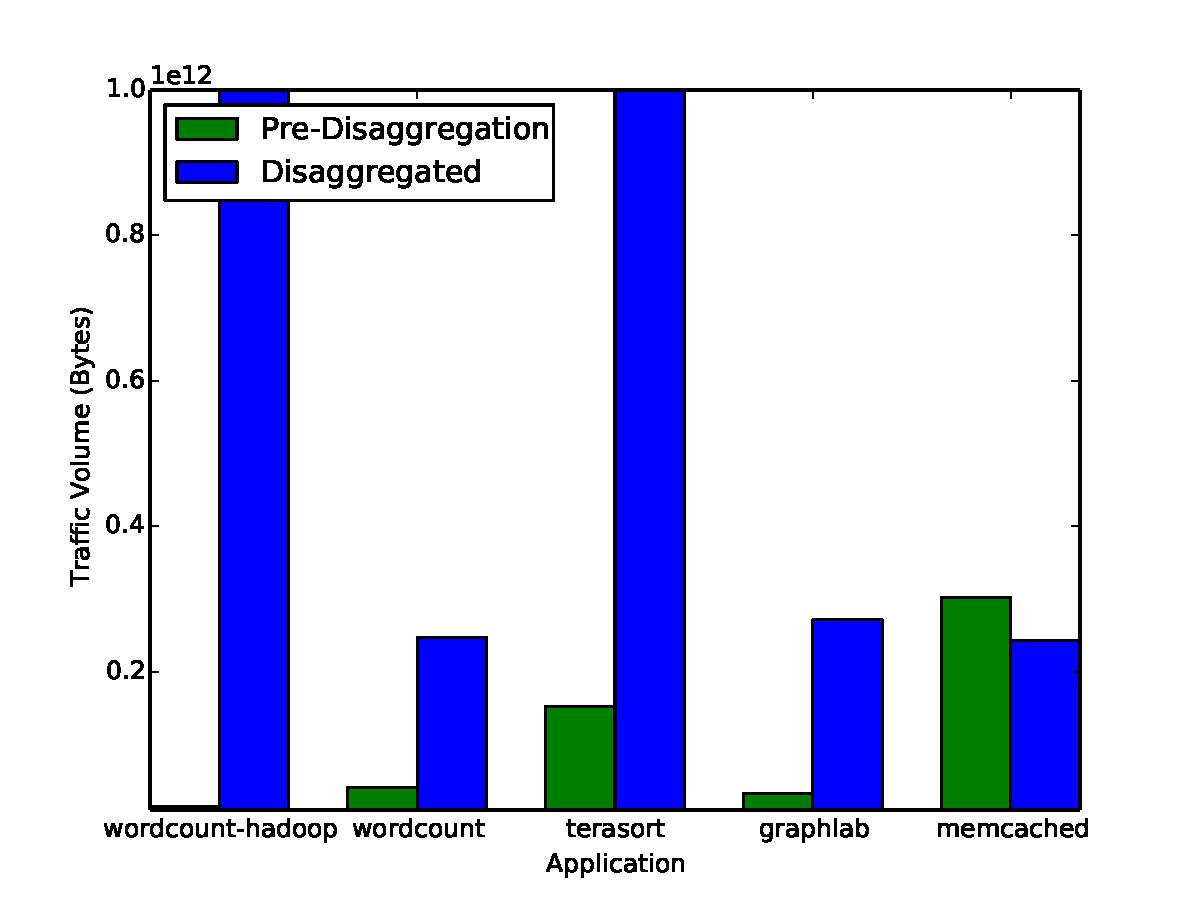
\includegraphics[width = 2.5in]{img/graph5_trafficvolume} 
  \caption{\small{Traffic volume in \dis and \pdis. Note that the y-axis is log-scaled.}}
  \label{fig:vol}
\end{figure}
%
\subsubsection{Traffic volume}
\label{sssec:tfvol}
We start with studying the traffic volume in \dis and \pdis (see Figure~\ref{fig:vol}). For most applications studied, the traffic volume in \dis increases due to the same reason the number of flows increases (shown in Figure~\ref{fig:nof}) --- intuitively, flows that previously were contained within a server are now carried over the network.

Just as memcached exhibits a greater number of flows in \pdis, its traffic volume is greater in \dis. Our experiments with 25\% of memory in the local cache, so we expect that approximately this amount of request traffic in memcached will be served from the local cache in \dis and avoid the network entirely. Accordingly, we observe that the difference in traffic volume between \dis and \pdis is 24\%. The difference in the number of flows is more drastic because the flow distributions are different --- while memcached in \pdis has a bimodal distribution of request and response flows of approximate size 30 bytes and 10KB respectively, in \dis the distribution varies in the range [4KB, 19MB]. The longer tail in flow sizes for \dis causes the drastic disparity in number of flows seen in Figure~\ref{fig:nof} despite a relatively modest increase in traffic volume.

% We note that the traffic volume in \dis is not much larger than in \pdis. At the first glance, this may seem rather surprising given the increase in traffic due to intra-server traffic becoming remote. However, note that memory accesses are just $4$KB in size; thus, a significantly large number of memory access traffic will correspond to a single long flow. Moreover, reads and writes that are local are only increased by a factor of $2\times$.
%
\begin{figure}[t]
  \centering
  \subfigure{
    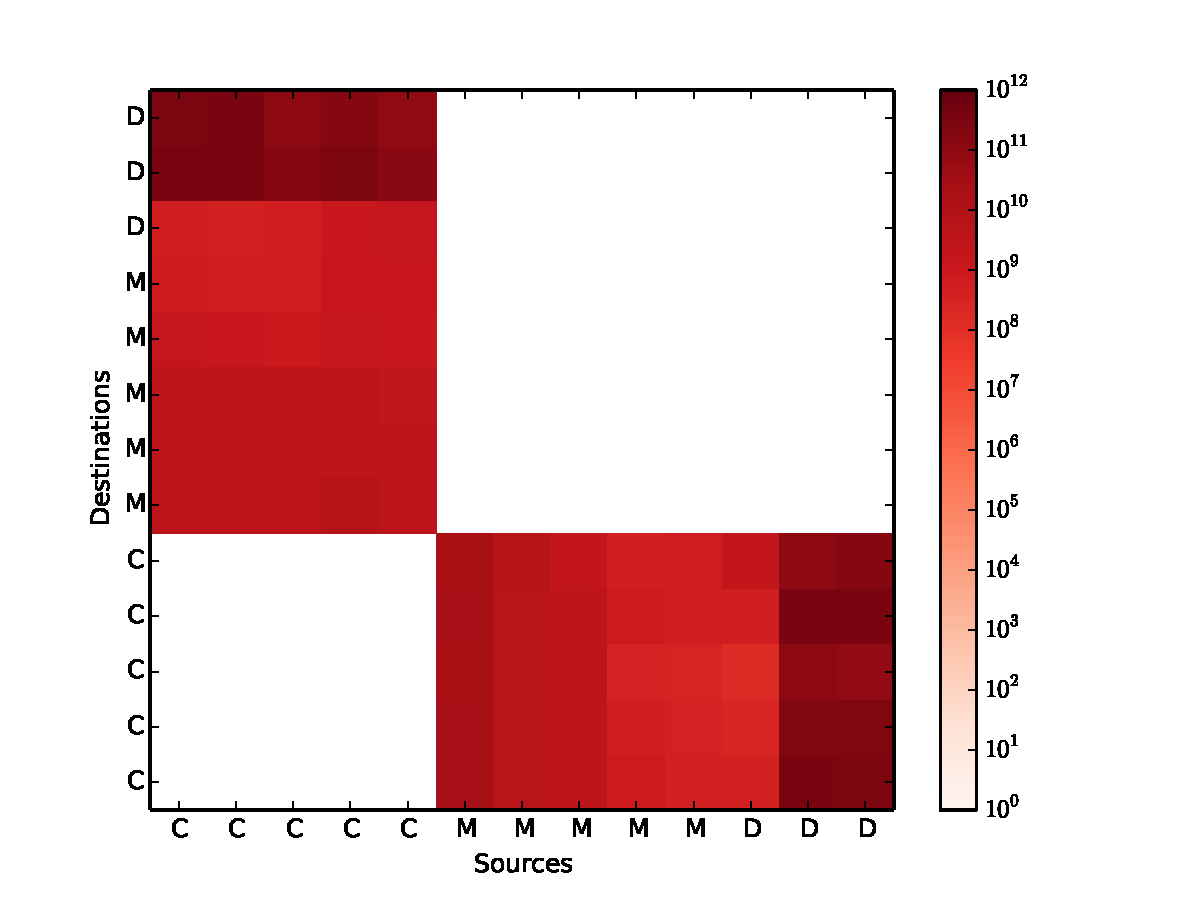
\includegraphics[width = 2.3in]{img/graph6_trafficvolumeheatmap_dis_terasort} 
	\label{fig:asdd}
  }
%\hspace{0.05in}
  \subfigure{
    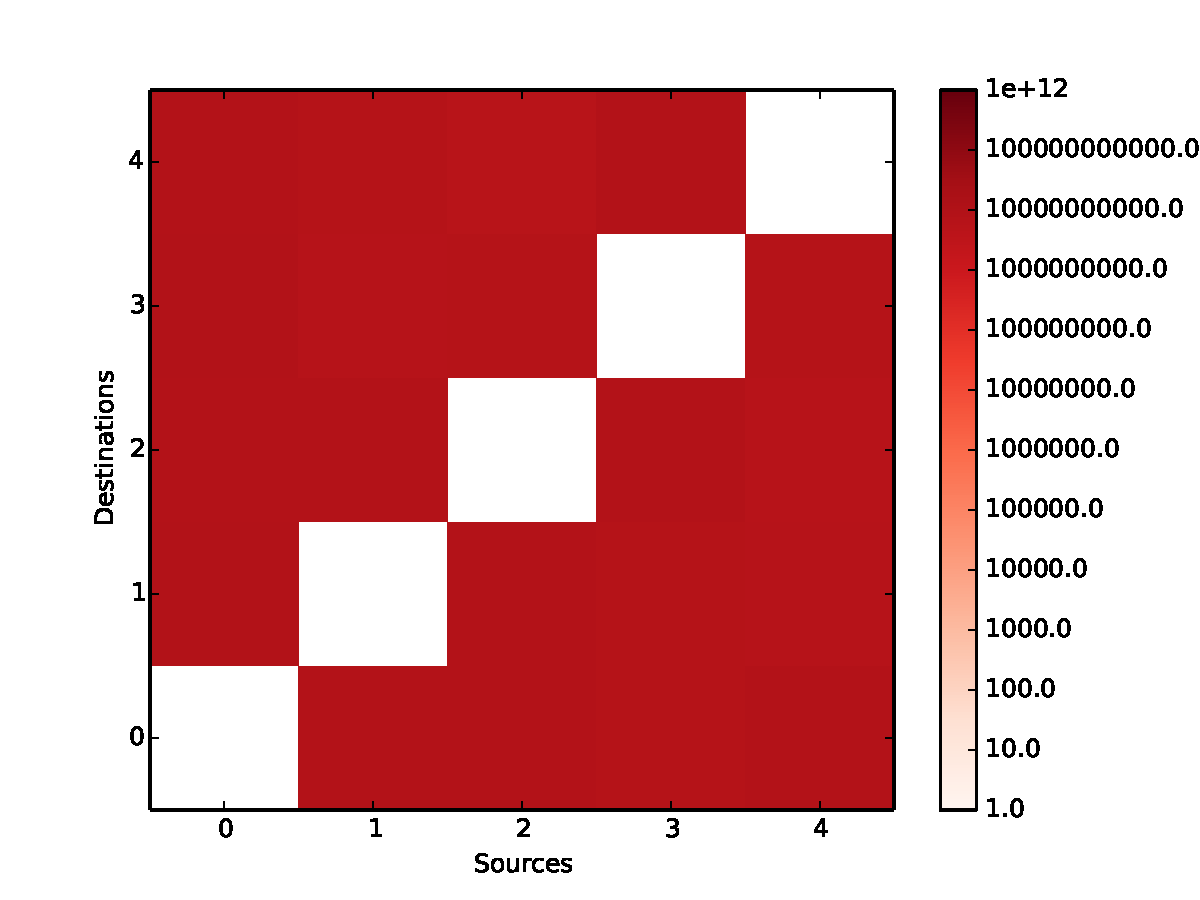
\includegraphics[width = 2.3in]{img/graph6_trafficvolumeheatmap_pdis_terasort}
	\label{fig:sdds}
  }
  \caption{\small{Spatial traffic distribution in \pdis and \dis for the terasort application. The x-axis represents senders and the y-axis receivers. In \pdis above, this is a $5 \times 5$ matrix for the 5 ec2 machines, while in \dis below, the heatmap is a $13 \times 13$ matrix, for the 5 cpu blades, 5 memory blades, and 3 disk blades we map the 5 ec2 machines to. For further details on this mapping see \S\ref{ssec:method1}.}}
  
  %A $n \times n$ matrix heat diagram, with cell $(i, j)$ having heat level corresponding to the traffic volume between source i and destination j. The same thing for \pdis.}}}
  \label{fig:sd}
\end{figure}
%
\subsubsection{Spatial distribution}
\label{sssec:spatialdist}
We now study the spatial distribution of traffic in \dis (see Figure~\ref{fig:sd}). Note that all traffic represented in Figure~\ref{fig:sdds} has a CPU as either its source or destination. This is a consequence of our assumption as discussed in \S~\ref{sec:summary} that CPUs do not share memory or disk resources. One could however imagine alternate models in which not all traffic is CPU-based. For example, disk accesses could be sent to the CPU that requested them while simultaneously being cached in remote memory. We leave an exploration of this design space to future work.

Also note that there are slightly more traffic volume to the first memory blades than to memory blades farther rightwards and upwards in the heatmap. Digging deeper, we found that lower memory addresses were more popular in the application shown, terasort (results for other applications are in . As a result, the memory blade that lower addresses were mapped to in our range hashing experienced a greater traffic volume from CPUs. This suggests that depending on the application's data access patterns, a different address mapping may be needed.
%First, when compared to \pdis, the traffic in \dis is significantly well distributed across the source-destination pairs. Indeed, the \dis architecture allows distributing a single read/write traffic across multiple nodes spatially distributed across the network. Second, the overall spatial distribution in \dis has significantly lower temperature than in \pdis, implying that on an average, each source-destination pair observes significantly lower traffic volume in \dis when compared to \pdis.

\subsubsection{Temporal distribution}
Finally, we study the temporal distribution of traffic in \dis and \pdis. Figure~\ref{fig:td} shows that, when compared to \pdis, the traffic distribution in \dis is significantly less bursty. This is because of an interesting effect caused by the data placement discussed in \S\ref{sec:summary}. When a long flow in \pdis is divided across multiple smaller flows in \dis (due to data placement across multiple disks), it is pipelined into multiple shorter flows. Akin to the task packing problem, where having multiple smaller tasks has a better packing compared to a single long task, dividing a single flow into multiple smaller flows ``packs'' into the network more efficiently, making traffic less bursty.
%
\begin{figure}[t]
  \centering
  \subfigure{
    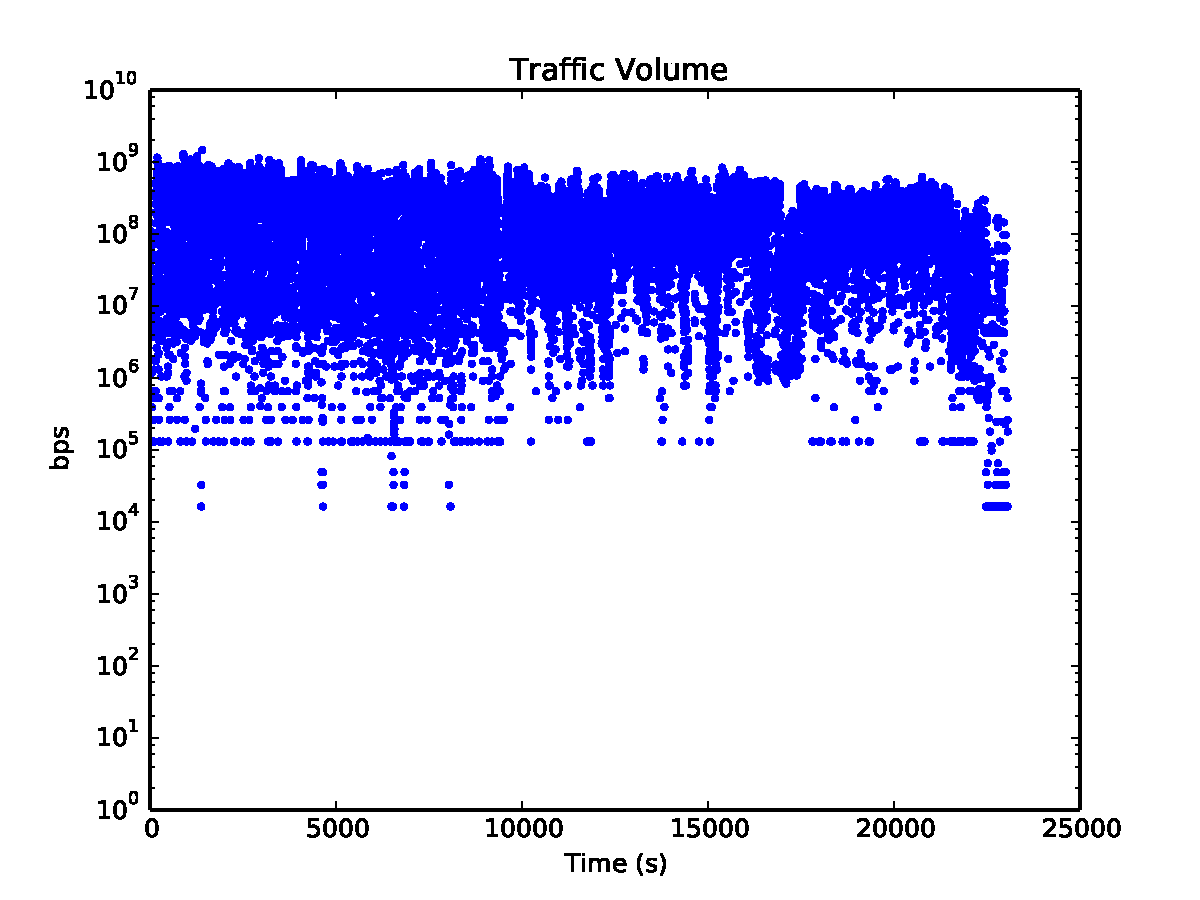
\includegraphics[width = 2.3in]{img/graph7_temporaltraffic_dis_terasort} 
	\label{fig:asdd}
  }
%\hspace{0.05in}
  \subfigure{
    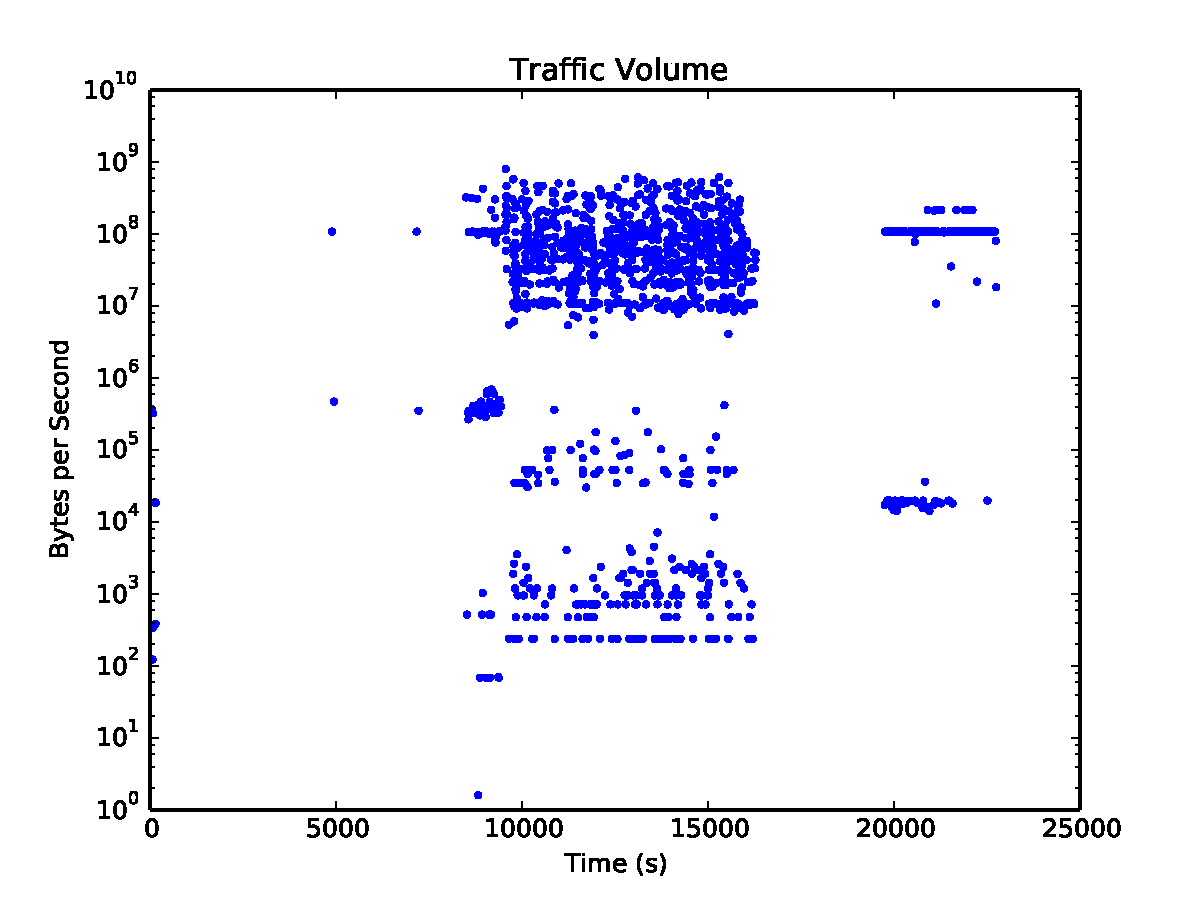
\includegraphics[width = 2.3in]{img/graph7_temporaltraffic_pdis_terasort}
	\label{fig:sdds}
  }
  \caption{\small{Temporal traffic distribution in \dis and \pdis for one of the applications. The trace was divided into 100ms timeslots, and flows were assigned to slots based on their start time. The traffic volume in these timeslots was then normalized to determine a value in bytes per second. Note the y-axis is log-scale.}}
  \label{fig:td}
\end{figure}
%

\subsubsection{Implications}
\label{ssec:implications}
\rc{Is this a valid implication?}
Overall, while we observed in \S\ref{sec:requirements} that low latencies are important for performance, we observe here that high bandwidths are not necessary to serve the volume of traffic injected into the network. Rather, we envision networks in \ddc being provisioned to meet \emph{latency} requirements, and being overprovisioned from a peak traffic volume perspective as a result. \rqc{more implications?} 

%\begin{itemize}[leftmargin=*]
%	\itemsep0em
%	\item Traffic volume --- do not need very high bandwidth networks
%	\item Spatial distribution --- traffic not so local
%	\item Temporal distribution --- do not need to design networks for peak traffic?
%\end{itemize}		

\subsection{Impact of design knobs}
\label{ssec:knobs}
We now study how various design parameters in \dis architecture design impact the observations made in this section. 

% \paragraphb{Impact of cache size} % discussed in section 3.
%\begin{figure}[t]
%\centering
%\subfigure{
%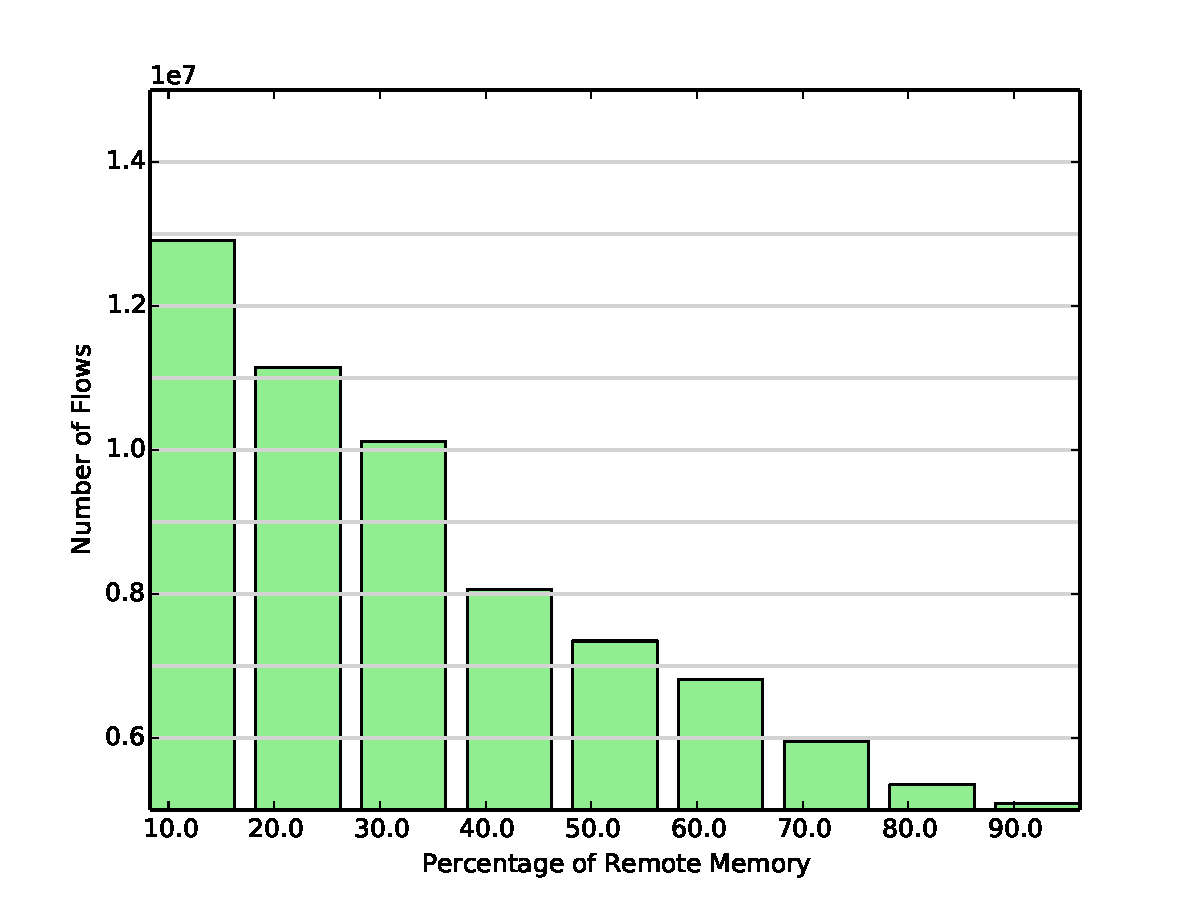
\includegraphics[width = 3.0in]{img/rmem_numflows}
%\label{fig:rmem_numflows}
%}
%\subfigure{
%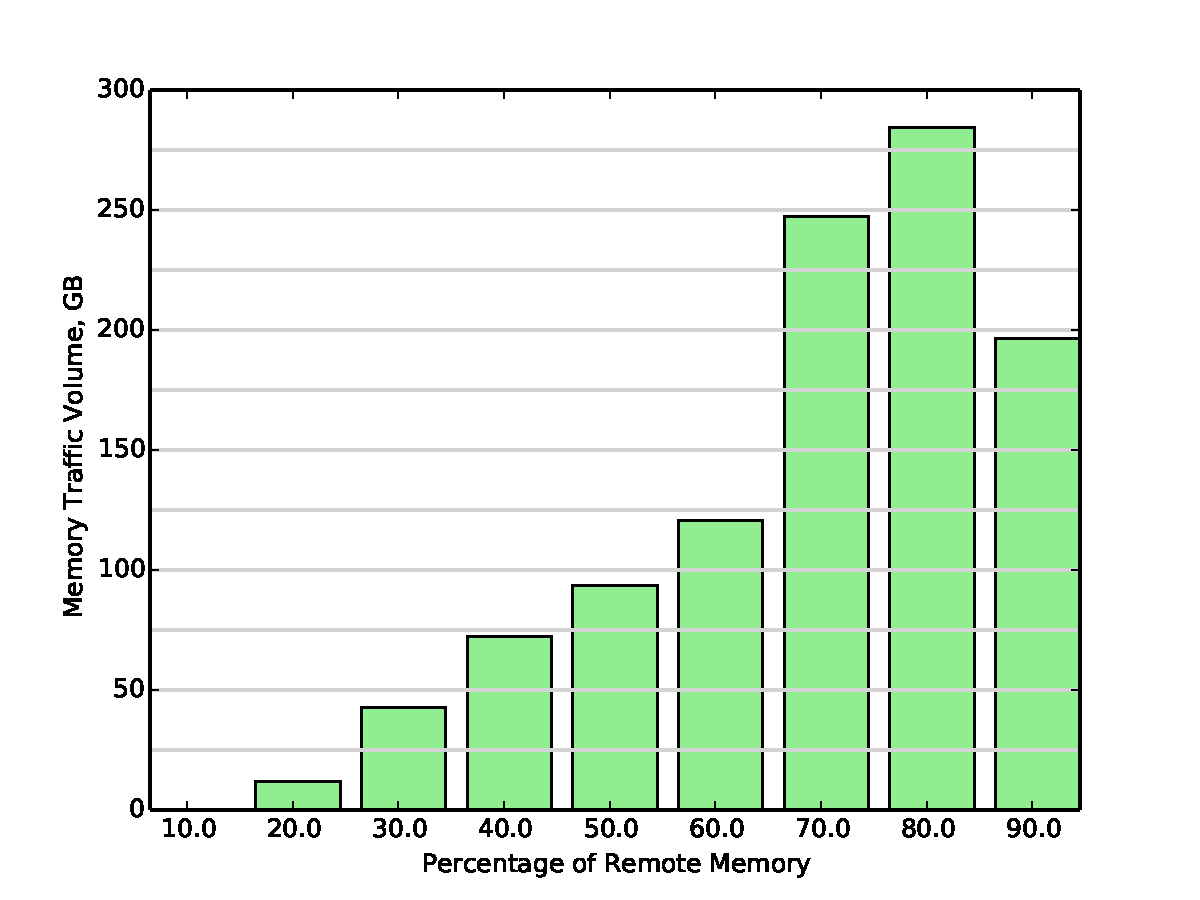
\includegraphics[width = 3.0in]{img/rmem_trafficvolume}
%\label{fig:rmem_trafvol}
%}
%\caption{Flow count (above) and traffic volume (below) with varying fraction of memory in the local cache.}
%\label{fig:rmem}
%\end{figure}

\paragraphb{Impact of remote versus local} 
\rqc{Peter's graphs showing performance of local disk vs remote memory}

\rc{what do these mean?}
    
\paragraphb{Impact of disaggregation scale}

\paragraphb{Impact of data placement}
